\PassOptionsToPackage{unicode=true}{hyperref} % options for packages loaded elsewhere
\PassOptionsToPackage{hyphens}{url}
%
\documentclass[]{article}
\usepackage{lmodern}
\usepackage{amssymb,amsmath}
\usepackage{ifxetex,ifluatex}
\usepackage{fixltx2e} % provides \textsubscript
\ifnum 0\ifxetex 1\fi\ifluatex 1\fi=0 % if pdftex
  \usepackage[T1]{fontenc}
  \usepackage[utf8]{inputenc}
  \usepackage{textcomp} % provides euro and other symbols
\else % if luatex or xelatex
  \usepackage{unicode-math}
  \defaultfontfeatures{Ligatures=TeX,Scale=MatchLowercase}
\fi
% use upquote if available, for straight quotes in verbatim environments
\IfFileExists{upquote.sty}{\usepackage{upquote}}{}
% use microtype if available
\IfFileExists{microtype.sty}{%
\usepackage[]{microtype}
\UseMicrotypeSet[protrusion]{basicmath} % disable protrusion for tt fonts
}{}
\IfFileExists{parskip.sty}{%
\usepackage{parskip}
}{% else
\setlength{\parindent}{0pt}
\setlength{\parskip}{6pt plus 2pt minus 1pt}
}
\usepackage{hyperref}
\hypersetup{
            pdfborder={0 0 0},
            breaklinks=true}
\urlstyle{same}  % don't use monospace font for urls
\usepackage{color}
\usepackage{fancyvrb}
\newcommand{\VerbBar}{|}
\newcommand{\VERB}{\Verb[commandchars=\\\{\}]}
\DefineVerbatimEnvironment{Highlighting}{Verbatim}{commandchars=\\\{\}}
% Add ',fontsize=\small' for more characters per line
\newenvironment{Shaded}{}{}
\newcommand{\AlertTok}[1]{\textcolor[rgb]{1.00,0.00,0.00}{\textbf{#1}}}
\newcommand{\AnnotationTok}[1]{\textcolor[rgb]{0.38,0.63,0.69}{\textbf{\textit{#1}}}}
\newcommand{\AttributeTok}[1]{\textcolor[rgb]{0.49,0.56,0.16}{#1}}
\newcommand{\BaseNTok}[1]{\textcolor[rgb]{0.25,0.63,0.44}{#1}}
\newcommand{\BuiltInTok}[1]{#1}
\newcommand{\CharTok}[1]{\textcolor[rgb]{0.25,0.44,0.63}{#1}}
\newcommand{\CommentTok}[1]{\textcolor[rgb]{0.38,0.63,0.69}{\textit{#1}}}
\newcommand{\CommentVarTok}[1]{\textcolor[rgb]{0.38,0.63,0.69}{\textbf{\textit{#1}}}}
\newcommand{\ConstantTok}[1]{\textcolor[rgb]{0.53,0.00,0.00}{#1}}
\newcommand{\ControlFlowTok}[1]{\textcolor[rgb]{0.00,0.44,0.13}{\textbf{#1}}}
\newcommand{\DataTypeTok}[1]{\textcolor[rgb]{0.56,0.13,0.00}{#1}}
\newcommand{\DecValTok}[1]{\textcolor[rgb]{0.25,0.63,0.44}{#1}}
\newcommand{\DocumentationTok}[1]{\textcolor[rgb]{0.73,0.13,0.13}{\textit{#1}}}
\newcommand{\ErrorTok}[1]{\textcolor[rgb]{1.00,0.00,0.00}{\textbf{#1}}}
\newcommand{\ExtensionTok}[1]{#1}
\newcommand{\FloatTok}[1]{\textcolor[rgb]{0.25,0.63,0.44}{#1}}
\newcommand{\FunctionTok}[1]{\textcolor[rgb]{0.02,0.16,0.49}{#1}}
\newcommand{\ImportTok}[1]{#1}
\newcommand{\InformationTok}[1]{\textcolor[rgb]{0.38,0.63,0.69}{\textbf{\textit{#1}}}}
\newcommand{\KeywordTok}[1]{\textcolor[rgb]{0.00,0.44,0.13}{\textbf{#1}}}
\newcommand{\NormalTok}[1]{#1}
\newcommand{\OperatorTok}[1]{\textcolor[rgb]{0.40,0.40,0.40}{#1}}
\newcommand{\OtherTok}[1]{\textcolor[rgb]{0.00,0.44,0.13}{#1}}
\newcommand{\PreprocessorTok}[1]{\textcolor[rgb]{0.74,0.48,0.00}{#1}}
\newcommand{\RegionMarkerTok}[1]{#1}
\newcommand{\SpecialCharTok}[1]{\textcolor[rgb]{0.25,0.44,0.63}{#1}}
\newcommand{\SpecialStringTok}[1]{\textcolor[rgb]{0.73,0.40,0.53}{#1}}
\newcommand{\StringTok}[1]{\textcolor[rgb]{0.25,0.44,0.63}{#1}}
\newcommand{\VariableTok}[1]{\textcolor[rgb]{0.10,0.09,0.49}{#1}}
\newcommand{\VerbatimStringTok}[1]{\textcolor[rgb]{0.25,0.44,0.63}{#1}}
\newcommand{\WarningTok}[1]{\textcolor[rgb]{0.38,0.63,0.69}{\textbf{\textit{#1}}}}
\usepackage{graphicx,grffile}
\makeatletter
\def\maxwidth{\ifdim\Gin@nat@width>\linewidth\linewidth\else\Gin@nat@width\fi}
\def\maxheight{\ifdim\Gin@nat@height>\textheight\textheight\else\Gin@nat@height\fi}
\makeatother
% Scale images if necessary, so that they will not overflow the page
% margins by default, and it is still possible to overwrite the defaults
% using explicit options in \includegraphics[width, height, ...]{}
\setkeys{Gin}{width=\maxwidth,height=\maxheight,keepaspectratio}
\setlength{\emergencystretch}{3em}  % prevent overfull lines
\providecommand{\tightlist}{%
  \setlength{\itemsep}{0pt}\setlength{\parskip}{0pt}}
\setcounter{secnumdepth}{0}
% Redefines (sub)paragraphs to behave more like sections
\ifx\paragraph\undefined\else
\let\oldparagraph\paragraph
\renewcommand{\paragraph}[1]{\oldparagraph{#1}\mbox{}}
\fi
\ifx\subparagraph\undefined\else
\let\oldsubparagraph\subparagraph
\renewcommand{\subparagraph}[1]{\oldsubparagraph{#1}\mbox{}}
\fi

% set default figure placement to htbp
\makeatletter
\def\fps@figure{htbp}
\makeatother


\date{}

\begin{document}

\hypertarget{header-n0}{%
\section{Sprawozdanie}\label{header-n0}}

Jakub Dymon, Paweł Nowacki, Paweł Sulżycki

\hypertarget{header-n4}{%
\subsection{Wstęp}\label{header-n4}}

\hypertarget{header-n5}{%
\subsubsection{Cele projektu}\label{header-n5}}

Celem projektu jest stworzenie aplikacji internetowej na potrzeby działu
kadr przedsiębiorstwa. Przedsiębiorstwo posiada trzy lokalizacje, a w
każdej z nich znajduje się dział kadr, który potrzebuje dostępu do
danych o wszystkich pracownikach firmy. Wszystkie lokalizacje są
równorzędne i potrzebują zarówno odczytywać, jak i edytować dane
pracowników.

\hypertarget{header-n8}{%
\subsubsection{Założenia projektowe}\label{header-n8}}

System pozwala na dodawanie i usuwanie pracowników, przeglądanie i
edycję danych osobowych pracowników i zależności hierarchicznych
pomiędzy nimi. Ponadto system replikacji bazy danych pozwala na obsługę
systemu z różnych oddziałów firmy rozsianych po całym świecie. System ma
formę aplikacji internetowej z systemem logowania i jest dostępny dla
odpowiednio przeszkolonych pracowników działu kadr. Konta użytkowników
są zakładane odgórnie przez administratora.

Aplikacja wykorzystuje relacyjną bazę danych MySQL oraz logikę biznesową
zaimplementowaną z użyciem języka Java i biblioteki Spring Framework
oraz pochodnych. Każda instancja aplikacji posiada własną bazę danych o
takich samej zawartości i jest dobierana na podstawie lokalizacji.
Stosowana jest replikacja migawkowa typu multimaster na poziomie bazy
danych i służy propagacji danych pomiędzy różnymi instancjami tej samej
aplikacji. Kontroli wersji danych służy mechanizm \emph{optimistic
locking}.

\hypertarget{header-n13}{%
\subsubsection{Zakres projektu}\label{header-n13}}

\hypertarget{header-n14}{%
\subsection{Replikacja w systemie baz danych MySQL}\label{header-n14}}

\hypertarget{header-n15}{%
\subsection{Modele baz danych}\label{header-n15}}

\hypertarget{header-n16}{%
\subsubsection{Model konceptualny}\label{header-n16}}

\begin{figure}
\centering
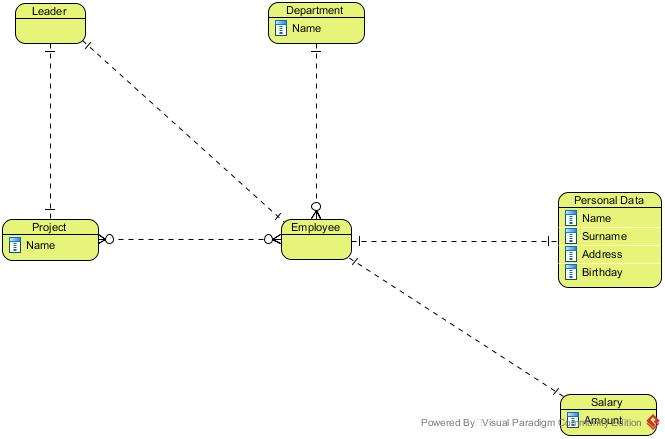
\includegraphics{C:/Users/Kuba/Documents/POLITECHNIKA/9. semestr/Bazy danych/projekt/Dokumentacja/ConceptualERD.jpg}
\caption{}
\end{figure}

\hypertarget{header-n19}{%
\subsubsection{Model logiczny}\label{header-n19}}

\begin{figure}
\centering
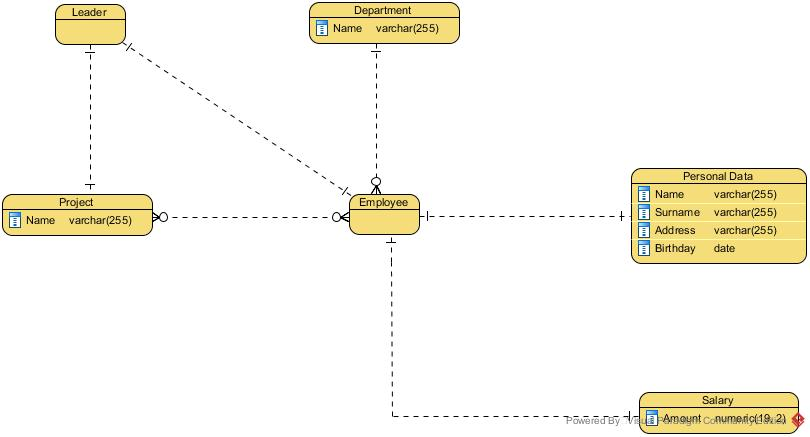
\includegraphics{C:/Users/Kuba/Documents/POLITECHNIKA/9. semestr/Bazy danych/projekt/Dokumentacja/LogicalERD.jpg}
\caption{}
\end{figure}

\hypertarget{header-n22}{%
\subsubsection{Model fizyczny}\label{header-n22}}

\begin{figure}
\centering
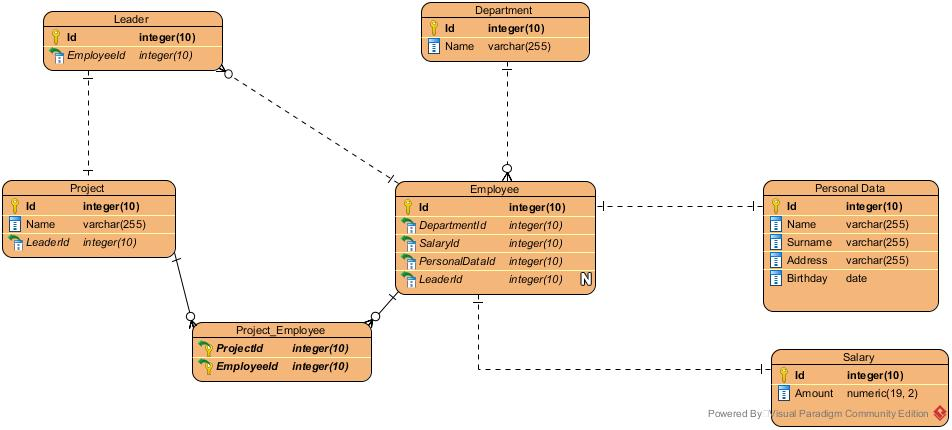
\includegraphics{C:/Users/Kuba/Documents/POLITECHNIKA/9. semestr/Bazy danych/projekt/Dokumentacja/PhysicalERD.jpg}
\caption{}
\end{figure}

\hypertarget{header-n25}{%
\subsection{Implementacja baz danych w środowisku
MySQL}\label{header-n25}}

\hypertarget{header-n26}{%
\subsubsection{Opis implementacji mechanizmu replikacyjnego
multi-master}\label{header-n26}}

Implementację mechanizmu replikacyjnego rozpoczęto od przygotowania
odpowiedniego środowiska, na którym będzie działać baza danych.

\hypertarget{header-n29}{%
\paragraph{Przygotowanie środowiska}\label{header-n29}}

\begin{enumerate}
\def\labelenumi{\arabic{enumi}.}
\item
  Instalacja VMware Workstation 14 Player na urządzeniu - hoście z
  systemem Windows
\item
  Instalacja maszyny wirtualnej z systemem Ubuntu 16.04 LTS
\item
  Instalacja najnowszej wersji MySQL.
\item
  Powielenie maszyny wirtualnej, tak aby otrzymać łącznie 3 maszyny.
\item
  Konfiguracja wirtualnej sieci lokalnej w celu umożliwienia komunikacji
  między maszynami. 
\end{enumerate}

\hypertarget{header-n46}{%
\paragraph{Konfiguracja maszyn wirtualnych}\label{header-n46}}

Kolejnym krokiem było konfiguracja maszyn wirtualnych w celu
umożliwienia replikacji.

\begin{enumerate}
\def\labelenumi{\arabic{enumi}.}
\item
  Dla każdej z maszyn wygenerowano unikalne ID grupy przy użyciu komendy

\begin{verbatim}
uuidgen
\end{verbatim}

  oraz sprawdzono adres IP maszyn przy użyciu

\begin{verbatim}
ifconfig
\end{verbatim}

  Zapisane dane potrzebne będą do dalszej konfiguracji.
\item
  Następnie utworzono pliki konfiguracyjne przy użyciu komendy

\begin{verbatim}
sudo gedit /etc/mysql/my.cnf
\end{verbatim}
\item
  Wypełnienie pliku konfiguracyjnego bazy danych według poniższego
  szablonu:

\begin{verbatim}
!includedir /etc/mysql/conf.d/
!includedir /etc/mysql/mysql.conf.d/

[mysqld]

# General replication settings
gtid_mode = ON
enforce_gtid_consistency = ON
master_info_repository = TABLE
relay_log_info_repository = TABLE
binlog_checksum = NONE
log_slave_updates = ON
log_bin = binlog
binlog_format = ROW
transaction_write_set_extraction = XXHASH64
loose-group_replication_bootstrap_group = OFF
loose-group_replication_start_on_boot = OFF
loose-group_replication_ssl_mode = REQUIRED
loose-group_replication_recovery_use_ssl = 1

# Shared replication group configuration
loose-group_replication_group_name = [wygenerowany id grupy]
loose-group_replication_ip_whitelist = [ip serwerów oddzielone ","]
loose-group_replication_group_seeds = [ip serwerów z portem 33061 oddzielone ","]

# Single or Multi-primary mode? Uncomment these two lines
# for multi-primary mode, where any host can accept writes
loose-group_replication_single_primary_mode = OFF
loose-group_replication_enforce_update_everywhere_checks = ON

# Host specific replication configuration
server_id = [id serwera]
bind-address = 127.0.0.1
report_host = [ip serwera]
loose-group_replication_local_address = [ip serwera]:33061
\end{verbatim}
\item
  Po zapisaniu pliku konfiguracyjnego należało zrestartować bazę danych
  przy użyciu komendy

\begin{verbatim}
sudo systemctl restart mysql
\end{verbatim}
\item
  Kolejnym krokiem było dodanie wyjątków do zapory sytemowej:

\begin{verbatim}
sudo ufw allow 33061
\end{verbatim}
\end{enumerate}

\hypertarget{header-n75}{%
\paragraph{Konfiguracja wewnątrz MySQL}\label{header-n75}}

\begin{enumerate}
\def\labelenumi{\arabic{enumi}.}
\item
  Po zalogowaniu się do bazy danych kolejnymi krokami były:
\item
  Utworzenie użytkownika bazy danych odpowiedzialnego za replikację
\item
  Instalacja pluginu umożliwiającego obsługę replikacji.
\item
  Po pomyślnej instalacji mechanizm replikacji był już praktycznie
  gotowy. Pozostało tylko utworzyć grupę baz danych:

\begin{verbatim}
SET GLOBAL group_replication_bootstrap_group=ON;
START GROUP_REPLICATION;
SET GLOBAL group_replication_bootstrap_group=OFF;
\end{verbatim}
\item
  Ostatnim krokiem było wystartowanie replikacji na pozostałych
  maszynach:

\begin{verbatim}
START GROUP_REPLICATION;
\end{verbatim}
\end{enumerate}

Poniżej widoczna jest tabela prezentująca bazy danych połączone w grupę
replikacji:

\begin{figure}
\centering
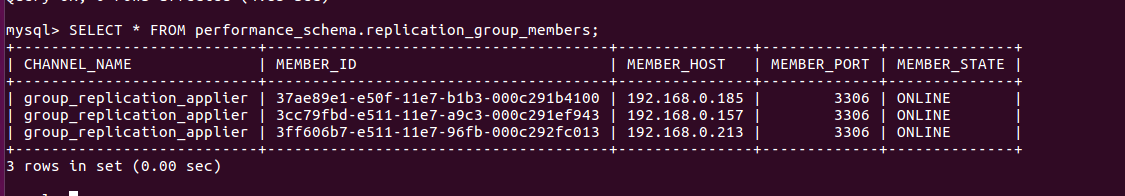
\includegraphics{C:/Users/Kuba/Documents/POLITECHNIKA/9. semestr/Bazy danych/projekt/Dokumentacja/group.PNG}
\caption{}
\end{figure}

Prezentacja działania mechanizmu replikacji dostępna jest w formie wideo
pod adresem: \url{https://youtu.be/CZzqGOR5zJk}.

\hypertarget{header-n100}{%
\subsubsection{Schemat bazy danych}\label{header-n100}}

Schemat bazy danych jest tworzony przez mechanizm HBM2DDL biblioteki
Hibernate na podstawie klas encji aplikacji klienckiej. Aby było to
możliwe należało skonfigurować aplikację z użyciem pliku
application.properties.

\begin{verbatim}
spring.datasource.url= jdbc:mysql://127.0.0.1:3306/hrs
spring.datasource.username=root
spring.datasource.password=admin
spring.datasource.driverClassName=com.mysql.jdbc.Driver
spring.jpa.show-sql=true
spring.jpa.hibernate.ddl-auto = create
spring.jpa.hibernate.naming.physical-strategy=org.springframework.boot.orm.jpa.hibernate.SpringPhysicalNamingStrategy
spring.jpa.properties.hibernate.hbm2ddl.import_files=import.sql
\end{verbatim}

Po skonfigurowaniu aplikacji należało stworzyć klasy encji, a następnie
uruchomić aplikację. Poniżej przedstawiono klasę encji reprezentującą
tabelę \emph{project}.

\begin{Shaded}
\begin{Highlighting}[]
\KeywordTok{package}\ImportTok{ hrs.database.project;}

\KeywordTok{import}\ImportTok{ hrs.database.employee.Employee;}
\KeywordTok{import}\ImportTok{ lombok.Getter;}
\KeywordTok{import}\ImportTok{ lombok.Setter;}

\KeywordTok{import}\ImportTok{ javax.persistence.*;}
\KeywordTok{import}\ImportTok{ javax.validation.constraints.NotNull;}
\KeywordTok{import}\ImportTok{ java.util.Collection;}

\AttributeTok{@Entity}
\AttributeTok{@Getter}
\AttributeTok{@Setter}
\KeywordTok{public} \KeywordTok{class}\NormalTok{ Project \{}

    \AttributeTok{@Id}
    \AttributeTok{@GeneratedValue}
    \KeywordTok{private} \BuiltInTok{Long}\NormalTok{ id;}

    \AttributeTok{@NotNull}
    \KeywordTok{private} \BuiltInTok{String}\NormalTok{ name;}

    \AttributeTok{@NotNull}
    \AttributeTok{@ManyToOne}
    \AttributeTok{@JoinColumn}
    \KeywordTok{private}\NormalTok{ Leader leader;}

    \AttributeTok{@NotNull}
    \AttributeTok{@ManyToMany}
    \AttributeTok{@JoinTable}\NormalTok{(name = }\StringTok{"project_employee"}\NormalTok{, joinColumns = \{}
            \AttributeTok{@JoinColumn}\NormalTok{(name = }\StringTok{"project_id"}\NormalTok{)}
\NormalTok{    \}, inverseJoinColumns = \{}
            \AttributeTok{@JoinColumn}\NormalTok{(name = }\StringTok{"employee_id"}\NormalTok{)}
\NormalTok{    \})}
    \KeywordTok{private} \BuiltInTok{Collection}\NormalTok{<Employee> employees;}

\NormalTok{\}}
\end{Highlighting}
\end{Shaded}

Kolumny tabeli reprezentowane są przez pola klasy, natomiast ich typ
definiuje typ zmiennej, a właściwości - adnotacje. Powyższa klasa
zawiera też definicję tabeli łączącej \emph{project\_employee}
zrealizowaną za pomocą adnotacji \emph{@JoinTable}.

\hypertarget{header-n109}{%
\subsection{Projekt i implementacja aplikacji
klienckiej}\label{header-n109}}

\hypertarget{header-n110}{%
\subsubsection{Funkcje aplikacji - diagram przypadków
użycia}\label{header-n110}}

Aplikacja realizuje przypadki użycia przedstawione na diagramie. Zostały
zaimplementowane jedynie wybrane funkcjonalności, które umożliwiają
zaprezentowanie działania mechanizmu replikacji.

\begin{figure}
\centering
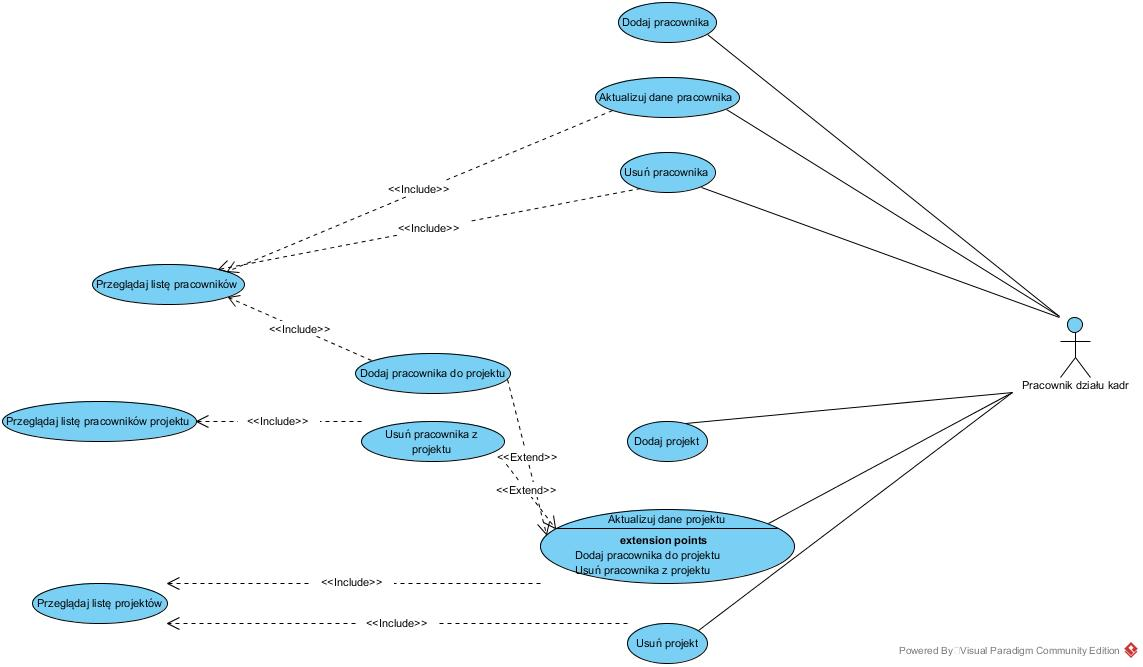
\includegraphics{C:/Users/Kuba/Documents/POLITECHNIKA/9. semestr/Bazy danych/projekt/Dokumentacja/Use Case Diagram.jpg}
\caption{}
\end{figure}

\hypertarget{header-n115}{%
\subsubsection{Realizacja wybranych funkcjonalności}\label{header-n115}}

W ramach projektu zrealizowano część aplikacji odpowiedzialną za
zarządzanie projektami, a więc przewidującą przypadki użycia: "dodaj
projekt", "aktualizuj dane projektu" i "usuń projekt" i ich nieodłączną
część "wyszukaj projekt".

\hypertarget{header-n118}{%
\paragraph{Wyszukiwanie projektu}\label{header-n118}}

Jak pokazano na diagramie przypadków użycia nieodłączną częścią
niektórych procesów jest wyszukiwanie projektu, które zostało
zrealizowane z użyciem biblioteki Spring Data JPA.

\begin{Shaded}
\begin{Highlighting}[]
\KeywordTok{package}\ImportTok{ hrs.database.project;}

\KeywordTok{import}\ImportTok{ org.springframework.data.jpa.repository.JpaRepository;}
\KeywordTok{import}\ImportTok{ org.springframework.data.jpa.repository.Query;}

\KeywordTok{import}\ImportTok{ java.util.List;}

\KeywordTok{public} \KeywordTok{interface}\NormalTok{ ProjectRepo }\KeywordTok{extends}\NormalTok{ JpaRepository<Project, }\BuiltInTok{Long}\NormalTok{> \{}

    \AttributeTok{@Query}\NormalTok{(}\StringTok{"select new hrs.database.project.ProjectListDO(p.id, p.name, p.leader.employee.personalData.name, p.leader.employee.personalData.surname, count(e)) from Project p left join p.employees as e group by p.id, p.name"}\NormalTok{)}
    \BuiltInTok{List}\NormalTok{<ProjectListDO> }\FunctionTok{findProjects}\NormalTok{();}

\NormalTok{\}}
\end{Highlighting}
\end{Shaded}

Wykonanie metody \emph{findProjects} jest równoznaczne z wykonaniem
zapytania JPQL podanego w adnotacji. Wartością zwracaną jest lista
obiektów typu \emph{ProjectListDO}.

\begin{Shaded}
\begin{Highlighting}[]
\KeywordTok{package}\ImportTok{ hrs.database.project;}

\KeywordTok{import}\ImportTok{ lombok.Getter;}
\KeywordTok{import}\ImportTok{ lombok.NoArgsConstructor;}
\KeywordTok{import}\ImportTok{ lombok.Setter;}

\AttributeTok{@Getter}
\AttributeTok{@Setter}
\AttributeTok{@NoArgsConstructor}
\KeywordTok{public} \KeywordTok{class}\NormalTok{ ProjectListDO \{}

    \KeywordTok{private} \BuiltInTok{Long}\NormalTok{ id;}

    \KeywordTok{private} \BuiltInTok{String}\NormalTok{ name;}

    \KeywordTok{private} \BuiltInTok{String}\NormalTok{ leader;}

    \KeywordTok{private} \BuiltInTok{Long}\NormalTok{ size;}

    \KeywordTok{public} \FunctionTok{ProjectListDO}\NormalTok{(}\BuiltInTok{Long}\NormalTok{ id, }\BuiltInTok{String}\NormalTok{ name, }\BuiltInTok{String}\NormalTok{ leaderName, }\BuiltInTok{String}\NormalTok{ leaderSurname, }\BuiltInTok{Long}\NormalTok{ size) \{}
        \KeywordTok{this}\NormalTok{.}\FunctionTok{id}\NormalTok{ = id;}
        \KeywordTok{this}\NormalTok{.}\FunctionTok{name}\NormalTok{ = name;}
        \KeywordTok{this}\NormalTok{.}\FunctionTok{leader}\NormalTok{ = leaderName + }\CharTok{' '}\NormalTok{ + leaderSurname;}
        \KeywordTok{this}\NormalTok{.}\FunctionTok{size}\NormalTok{ = size;}
\NormalTok{    \}}
\NormalTok{\}}
\end{Highlighting}
\end{Shaded}

Następnie lista jest udostępniana użytkownikowi przez punkt dostępu typu
REST zdefiniowany w metodzie \emph{findProjects} klasy
\emph{ProjectListResource}.

\begin{Shaded}
\begin{Highlighting}[]
\KeywordTok{package}\ImportTok{ hrs.rest.employee;}

\KeywordTok{import}\ImportTok{ hrs.database.project.ProjectRepo;}
\KeywordTok{import}\ImportTok{ org.springframework.beans.factory.annotation.Autowired;}
\KeywordTok{import}\ImportTok{ org.springframework.stereotype.Controller;}
\KeywordTok{import}\ImportTok{ org.springframework.ui.Model;}
\KeywordTok{import}\ImportTok{ org.springframework.web.bind.annotation.RequestMapping;}
\KeywordTok{import}\ImportTok{ org.springframework.web.bind.annotation.RequestParam;}

\AttributeTok{@Controller}
\AttributeTok{@RequestMapping}\NormalTok{(}\StringTok{"/project"}\NormalTok{)}
\KeywordTok{public} \KeywordTok{class}\NormalTok{ ProjectListResource \{}

    \AttributeTok{@Autowired}
    \KeywordTok{private}\NormalTok{ ProjectRepo projectRepo;}

    \AttributeTok{@RequestMapping}
    \KeywordTok{public} \BuiltInTok{String} \FunctionTok{findProjects}\NormalTok{(Model model) \{}
\NormalTok{        model.}\FunctionTok{addAttribute}\NormalTok{(}\StringTok{"projects"}\NormalTok{, projectRepo.}\FunctionTok{findProjects}\NormalTok{());}
        \KeywordTok{return} \StringTok{"project-list"}\NormalTok{;}
\NormalTok{    \}}

\NormalTok{\}}
\end{Highlighting}
\end{Shaded}

Wartością zwracaną metody jest nazwa szablonu strony internetowej, która
ma zostać pokazana w przeglądarce w odpowiedzi na zapytanie metodą GET
na adres \emph{\textless{}host\textgreater{}/project}. Szablon zostanie
wypełniony danymi przekazanymi jako atrybut modelu o nazwie
\emph{projects}. Za połączenie modelu i widoku odpowiada biblioteka
Thymeleaf. W szablonie zastosowano także bibliotekę Bootstrap,
dostarczającą gotowych komponentów.

\begin{Shaded}
\begin{Highlighting}[]
\KeywordTok{<html}\OtherTok{ xmlns=}\StringTok{"http://www.w3.org/1999/xhtml"}
\OtherTok{      xmlns:th=}\StringTok{"http://www.thymeleaf.org"}
\KeywordTok{>}
\KeywordTok{<head>}
    \KeywordTok{<meta}\OtherTok{ charset=}\StringTok{"utf-8"}\KeywordTok{/>}
    \KeywordTok{<title>}\NormalTok{HRS}\KeywordTok{</title>}
    \KeywordTok{<link}\OtherTok{ th:href=}\StringTok{"@\{~/bootstrap/css/bootstrap.min.css\}"}\OtherTok{ rel=}\StringTok{"stylesheet"}\KeywordTok{>}
    \KeywordTok{<link}\OtherTok{ th:href=}\StringTok{"@\{~/css/main.css\}"}\OtherTok{ rel=}\StringTok{"stylesheet"}\KeywordTok{>}
\KeywordTok{</head>}
\KeywordTok{<body>}
\KeywordTok{<div}\OtherTok{ class=}\StringTok{"container"}\KeywordTok{>}
    \KeywordTok{<div}\OtherTok{ class=}\StringTok{"row"}\KeywordTok{>}
        \KeywordTok{<div}\OtherTok{ class=}\StringTok{"col-md-12"}\KeywordTok{>}
            \KeywordTok{<a}\OtherTok{ href=}\StringTok{"/project/create"}\OtherTok{ class=}\StringTok{"btn btn-success"}\OtherTok{ role=}\StringTok{"button"}\KeywordTok{>}\NormalTok{Dodaj projekt}\KeywordTok{</a>}
        \KeywordTok{</div>}
    \KeywordTok{</div>}
    \KeywordTok{<div}\OtherTok{ class=}\StringTok{"row"}\KeywordTok{>}
        \KeywordTok{<div}\OtherTok{ class=}\StringTok{"col-md-12"}\KeywordTok{>}
            \KeywordTok{<table}\OtherTok{ class=}\StringTok{"table-striped"}\KeywordTok{>}
                \KeywordTok{<thead>}
                \KeywordTok{<th>}\NormalTok{Nazwa}\KeywordTok{</th>}
                \KeywordTok{<th>}\NormalTok{Kierownik}\KeywordTok{</th>}
                \KeywordTok{<th>}\NormalTok{Liczba pracowników</th>}
                \KeywordTok{<th></th>}
                \KeywordTok{<th></th>}
                \KeywordTok{</thead>}
                \KeywordTok{<tbody>}
                \KeywordTok{<tr}\OtherTok{ th:each=}\StringTok{"project : $\{projects\}"}\KeywordTok{>}
                    \KeywordTok{<td}\OtherTok{ th:text=}\StringTok{"$\{project.name\}"}\KeywordTok{></td>}
                    \KeywordTok{<td}\OtherTok{ th:text=}\StringTok{"$\{project.leader\}"}\KeywordTok{></td>}
                    \KeywordTok{<td}\OtherTok{ th:text=}\StringTok{"$\{project.size\}"}\KeywordTok{></td>}
                    \KeywordTok{<td>}
                        \KeywordTok{<a}\OtherTok{ th:href=}\StringTok{"'/project/edit?id=' + $\{project.id\}"}\OtherTok{ class=}\StringTok{"btn btn-info"}\OtherTok{ role=}\StringTok{"button"}\KeywordTok{>}\NormalTok{Edytuj}\KeywordTok{</a>}
                    \KeywordTok{</td>}
                    \KeywordTok{<td>}
                        \KeywordTok{<a}\OtherTok{ th:href=}\StringTok{"'/project/remove?id=' + $\{project.id\}"}\OtherTok{ class=}\StringTok{"btn btn-danger"}\OtherTok{ role=}\StringTok{"button"}\KeywordTok{>}\NormalTok{Usuń}\KeywordTok{</a>}
                    \KeywordTok{</td>}
                \KeywordTok{</tr>}
                \KeywordTok{</tbody>}
            \KeywordTok{</table>}
        \KeywordTok{</div>}
    \KeywordTok{</div>}
    \KeywordTok{<script}\OtherTok{ th:src=}\StringTok{"@\{~/jquery/jquery-3.2.1.min.js\}"}\KeywordTok{></script>}
    \KeywordTok{<script}\OtherTok{ th:src=}\StringTok{"@\{~/bootstrap/js/bootstrap.min.js\}"}\KeywordTok{></script>}
\KeywordTok{</div>}
\KeywordTok{</body>}
\KeywordTok{</html>}
\end{Highlighting}
\end{Shaded}

Po otwarciu adresu \url{http://localhost:8080/project} można przeglądać
listę projektów.

\begin{figure}
\centering
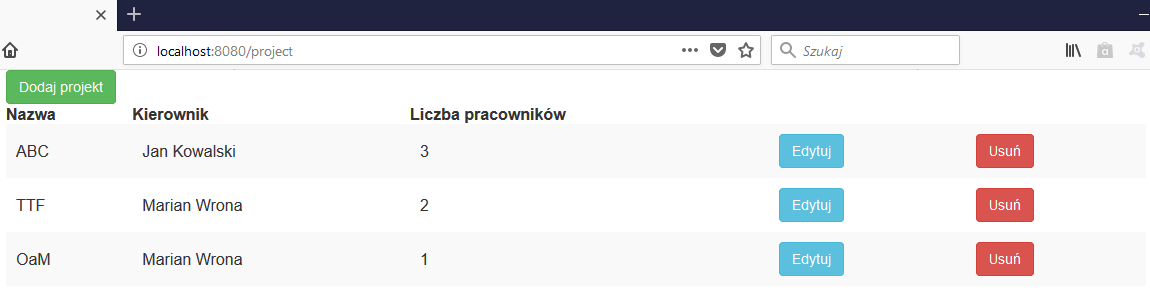
\includegraphics{C:/Users/Kuba/Documents/POLITECHNIKA/9. semestr/Bazy danych/projekt/Dokumentacja/Lista.PNG}
\caption{}
\end{figure}

\hypertarget{header-n135}{%
\paragraph{Usuwanie projektów}\label{header-n135}}

Jak można zauważyć w kodzie szablonu naciśnięcie przycisku \emph{Usuń}
wywoła wysłanie zapytania typu GET na adres
\emph{\textless{}host\textgreater{}/project?remove=\textless{}id\textgreater{}},
gdzie \emph{id} zostanie zastąpione odpowiednią wartością. Aby możliwe
było odebranie zapytania, należało zdefiniować w klasie
\emph{ProjectListResource} kolejny punkt dostępu, reprezentowany metodą
\emph{removeProject}.

\begin{Shaded}
\begin{Highlighting}[]
\AttributeTok{@RequestMapping}\NormalTok{(}\StringTok{"/remove"}\NormalTok{)}
\KeywordTok{public} \BuiltInTok{String} \FunctionTok{removeProject}\NormalTok{(}\AttributeTok{@RequestParam}\NormalTok{(}\StringTok{"id"}\NormalTok{) }\BuiltInTok{Long}\NormalTok{ id)\{}
\NormalTok{  projectRepo.}\FunctionTok{delete}\NormalTok{(id);}
  \KeywordTok{return} \StringTok{"redirect:/project"}\NormalTok{;}
\NormalTok{\}}
\end{Highlighting}
\end{Shaded}

Metoda przyjmuje id jako parametr i usuwa z bazy odpowiedni rekord z
pomocą metody \emph{delete} zdefiniowanej w klasie \emph{ProjectRepo}
przez interfejs \emph{JpaRepository} pochodzący z biblioteki Spring Data
JPA. Nie trzeba więc tworzyć zapytania samodzielnie. Po wykonaniu
usuwania aplikacja przekierowuje na adres
\emph{\textless{}host\textgreater{}/project}, gdzie użytkownik może
zobaczyć zaktualizowaną listę projektów.

\hypertarget{header-n141}{%
\paragraph{Edytowanie danych projektu}\label{header-n141}}

Aby możliwe było edytowanie danych projektu należało stworzyć nowy
szablon definiujący odpowiedni formularz.

\begin{Shaded}
\begin{Highlighting}[]
\KeywordTok{<html}\OtherTok{ xmlns=}\StringTok{"http://www.w3.org/1999/xhtml"}
\OtherTok{      xmlns:th=}\StringTok{"http://www.thymeleaf.org"}
\KeywordTok{>}
\KeywordTok{<head>}
    \KeywordTok{<meta}\OtherTok{ charset=}\StringTok{"utf-8"}\KeywordTok{/>}
    \KeywordTok{<title>}\NormalTok{HRS}\KeywordTok{</title>}
    \KeywordTok{<link}\OtherTok{ th:href=}\StringTok{"@\{~/bootstrap/css/bootstrap.min.css\}"}\OtherTok{ rel=}\StringTok{"stylesheet"}\KeywordTok{>}
    \KeywordTok{<link}\OtherTok{ th:href=}\StringTok{"@\{~/css/main.css\}"}\OtherTok{ rel=}\StringTok{"stylesheet"}\KeywordTok{>}
\KeywordTok{</head>}
\KeywordTok{<body>}
\KeywordTok{<div}\OtherTok{ class=}\StringTok{"container"}\KeywordTok{>}
    \KeywordTok{<div}\OtherTok{ class=}\StringTok{"row"}\KeywordTok{>}
        \KeywordTok{<div}\OtherTok{ class=}\StringTok{"col-md-12"}\KeywordTok{>}
            \KeywordTok{<h2}\OtherTok{ th:text=}\StringTok{"$\{activity\}"}\KeywordTok{></h2>}
        \KeywordTok{</div>}
    \KeywordTok{</div>}
    \KeywordTok{<div}\OtherTok{ class=}\StringTok{"row"}\KeywordTok{>}
        \KeywordTok{<div}\OtherTok{ class=}\StringTok{"col-md-12"}\KeywordTok{>}
            \KeywordTok{<form}\OtherTok{ action=}\StringTok{"/project/save"}\OtherTok{ method=}\StringTok{"POST"}\OtherTok{ id=}\StringTok{"edit-form"}\OtherTok{ th:object=}\StringTok{"$\{project\}"}\KeywordTok{>}
                \KeywordTok{<input}\OtherTok{ type=}\StringTok{"hidden"}\OtherTok{ name=}\StringTok{"id"}\OtherTok{ th:value=}\StringTok{"*\{id\}"}\KeywordTok{>}
                \KeywordTok{<div}\OtherTok{ class=}\StringTok{"form-group"}\KeywordTok{>}
                    \KeywordTok{<label}\OtherTok{ class=}\StringTok{"control-label col-sm-2"}\OtherTok{ for=}\StringTok{"name"}\KeywordTok{>}\NormalTok{Nazwa*:}\KeywordTok{</label>}
                    \KeywordTok{<div}\OtherTok{ class=}\StringTok{"col-sm-10"}\KeywordTok{>}
                        \KeywordTok{<input}\OtherTok{ type=}\StringTok{"text"}\OtherTok{ class=}\StringTok{"form-control"}\OtherTok{ id=}\StringTok{"name"}\OtherTok{ name=}\StringTok{"name"}\OtherTok{ th:value=}\StringTok{"*\{name\}"}
\OtherTok{                               required}\KeywordTok{>}
                    \KeywordTok{</div>}
                \KeywordTok{</div>}
                \KeywordTok{<div}\OtherTok{ class=}\StringTok{"form-group"}\KeywordTok{>}
                    \KeywordTok{<label}\OtherTok{ class=}\StringTok{"control-label col-sm-2"}\OtherTok{ for=}\StringTok{"leaderCandidateId"}\KeywordTok{>}\NormalTok{Kierownik*:}\KeywordTok{</label>}
                    \KeywordTok{<div}\OtherTok{ class=}\StringTok{"col-sm-10"}\KeywordTok{>}
                        \KeywordTok{<select}\OtherTok{ name=}\StringTok{"leaderCandidateId"}\OtherTok{ id=}\StringTok{"leaderCandidateId"}\OtherTok{ th:field=}\StringTok{"*\{leaderCandidateId\}"}\KeywordTok{>}
                            \KeywordTok{<option}\OtherTok{ th:each=}\StringTok{"employee : $\{employees\}"}
\OtherTok{                                    th:value=}\StringTok{"$\{employee.id\}"}
\OtherTok{                                    th:text=}\StringTok{"$\{employee.name\}"}\KeywordTok{></option>}
                        \KeywordTok{</select>}
                    \KeywordTok{</div>}
                \KeywordTok{</div>}
                \KeywordTok{<button}\OtherTok{ type=}\StringTok{"submit"}\OtherTok{ class=}\StringTok{"btn btn-success"}\KeywordTok{>}\NormalTok{Zapisz}\KeywordTok{</button>}
                \KeywordTok{<a}\OtherTok{ href=}\StringTok{"/project"}\OtherTok{ class=}\StringTok{"btn btn-warning"}\OtherTok{ role=}\StringTok{"button"}\KeywordTok{>}\NormalTok{Anuluj}\KeywordTok{</a>}
        \KeywordTok{</div>}
        \KeywordTok{</form>}
    \KeywordTok{</div>}
\KeywordTok{</div>}
\KeywordTok{<script}\OtherTok{ th:src=}\StringTok{"@\{~/jquery/jquery-3.2.1.min.js\}"}\KeywordTok{></script>}
\KeywordTok{<script}\OtherTok{ th:src=}\StringTok{"@\{~/bootstrap/js/bootstrap.min.js\}"}\KeywordTok{></script>}
\KeywordTok{<script}\OtherTok{ th:src=}\StringTok{"@\{~/js/person-edit.js\}"}\KeywordTok{></script>}
\KeywordTok{</div>}
\KeywordTok{</body>}
\KeywordTok{</html>}
\end{Highlighting}
\end{Shaded}

Szablon zawiera formularz składający się z pola tekstowego zawierającego
nazwę projektu oraz listy rozwijanej pozwalającej na wybór pracownika
mającego zostać liderem. Do obsługi stworzonego szablonu w klasie
\emph{ProjectEditResource} zdefiniowano dwa nowe punkty dostępu:

\begin{itemize}
\item
  do odczytu danych edytowanego projektu - GET
  \emph{\textless{}host\textgreater{}/project/edit?id=\textless{}id\textgreater{}}
\item
  do zapisu zmian - POST
  \emph{\textless{}host\textgreater{}/project/save}
\end{itemize}

\begin{Shaded}
\begin{Highlighting}[]
\KeywordTok{package}\ImportTok{ hrs.rest.employee;}

\KeywordTok{import}\ImportTok{ hrs.database.employee.Employee;}
\KeywordTok{import}\ImportTok{ hrs.database.employee.LeaderCandidateDO;}
\KeywordTok{import}\ImportTok{ hrs.database.employee.EmployeeRepo;}
\KeywordTok{import}\ImportTok{ hrs.database.project.*;}
\KeywordTok{import}\ImportTok{ org.springframework.beans.factory.annotation.Autowired;}
\KeywordTok{import}\ImportTok{ org.springframework.stereotype.Controller;}
\KeywordTok{import}\ImportTok{ org.springframework.ui.Model;}
\KeywordTok{import}\ImportTok{ org.springframework.web.bind.annotation.ModelAttribute;}
\KeywordTok{import}\ImportTok{ org.springframework.web.bind.annotation.RequestMapping;}
\KeywordTok{import}\ImportTok{ org.springframework.web.bind.annotation.RequestMethod;}
\KeywordTok{import}\ImportTok{ org.springframework.web.bind.annotation.RequestParam;}

\KeywordTok{import}\ImportTok{ java.util.List;}

\AttributeTok{@Controller}
\AttributeTok{@RequestMapping}\NormalTok{(}\StringTok{"/project"}\NormalTok{)}
\KeywordTok{public} \KeywordTok{class}\NormalTok{ ProjectEditController \{}

    \AttributeTok{@Autowired}
    \KeywordTok{private}\NormalTok{ ProjectRepo projectRepo;}

    \AttributeTok{@Autowired}
    \KeywordTok{private}\NormalTok{ EmployeeRepo employeeRepo;}

    \AttributeTok{@Autowired}
    \KeywordTok{private}\NormalTok{ LeaderRepo leaderRepo;}

    \AttributeTok{@RequestMapping}\NormalTok{(}\StringTok{"/edit"}\NormalTok{)}
    \KeywordTok{public} \BuiltInTok{String} \FunctionTok{openProject}\NormalTok{(}\AttributeTok{@RequestParam}\NormalTok{(}\StringTok{"id"}\NormalTok{) }\BuiltInTok{Long}\NormalTok{ id, Model model)\{}
\NormalTok{        ProjectEditDO project = }\KeywordTok{new} \FunctionTok{ProjectEditDO}\NormalTok{(projectRepo.}\FunctionTok{findOne}\NormalTok{(id));}
\NormalTok{        model.}\FunctionTok{addAttribute}\NormalTok{(}\StringTok{"project"}\NormalTok{, project);}
        \BuiltInTok{List}\NormalTok{<LeaderCandidateDO> leaderCandidates = employeeRepo.}\FunctionTok{findLeaderCandidates}\NormalTok{();}
\NormalTok{        model.}\FunctionTok{addAttribute}\NormalTok{(}\StringTok{"employees"}\NormalTok{, leaderCandidates);}
\NormalTok{        model.}\FunctionTok{addAttribute}\NormalTok{(}\StringTok{"activity"}\NormalTok{, }\StringTok{"Edytuj projekt"}\NormalTok{);}
        \KeywordTok{return} \StringTok{"project-edit"}\NormalTok{;}
\NormalTok{    \}}

    \AttributeTok{@RequestMapping}\NormalTok{(value = }\StringTok{"/save"}\NormalTok{, method = RequestMethod.}\FunctionTok{POST}\NormalTok{)}
    \KeywordTok{public} \BuiltInTok{String} \FunctionTok{saveProject}\NormalTok{(}\AttributeTok{@ModelAttribute}\NormalTok{(}\StringTok{"project"}\NormalTok{) ProjectEditDO projectData) \{}
\NormalTok{        Project project = projectRepo.}\FunctionTok{findOne}\NormalTok{(projectData.}\FunctionTok{getId}\NormalTok{());}
\NormalTok{        project.}\FunctionTok{setName}\NormalTok{(projectData.}\FunctionTok{getName}\NormalTok{());}
        \KeywordTok{if}\NormalTok{ (project.}\FunctionTok{getLeader}\NormalTok{().}\FunctionTok{getEmployee}\NormalTok{().}\FunctionTok{getId}\NormalTok{() != projectData.}\FunctionTok{getLeaderCandidateId}\NormalTok{()) \{}
\NormalTok{            Leader formerLeader = project.}\FunctionTok{getLeader}\NormalTok{();}
\NormalTok{            project.}\FunctionTok{setLeader}\NormalTok{(}\FunctionTok{createLeader}\NormalTok{(projectData));}
\NormalTok{            projectRepo.}\FunctionTok{save}\NormalTok{(project);}
\NormalTok{            leaderRepo.}\FunctionTok{delete}\NormalTok{(formerLeader);}
\NormalTok{        \} }\KeywordTok{else}\NormalTok{ \{}
\NormalTok{            projectRepo.}\FunctionTok{save}\NormalTok{(project);}
\NormalTok{        \}}
        \KeywordTok{return} \StringTok{"redirect:/project"}\NormalTok{;}
\NormalTok{    \}}

    \KeywordTok{private}\NormalTok{ Leader }\FunctionTok{createLeader}\NormalTok{(}\AttributeTok{@ModelAttribute}\NormalTok{(}\StringTok{"project"}\NormalTok{) ProjectEditDO projectData) \{}
\NormalTok{        Employee chosenLeader = employeeRepo.}\FunctionTok{findOne}\NormalTok{(projectData.}\FunctionTok{getLeaderCandidateId}\NormalTok{());}
        \KeywordTok{return}\NormalTok{ leaderRepo.}\FunctionTok{save}\NormalTok{(}\KeywordTok{new} \FunctionTok{Leader}\NormalTok{(chosenLeader));}
\NormalTok{    \}}

\NormalTok{\}}
\end{Highlighting}
\end{Shaded}

W przypadku odczytu danych oprócz danych samego projektu pobierana jest
lista pracowników - potencjalnych liderów - służąca wypełnieniu listy
rozwijanej. Zapis polega natomiast na uzupełnieniu odpowiednich
atrybutów encji - a także, jeśli to konieczne, stworzeniu rekordu nowego
lidera i usunięciu starego. Ponownie operacje te są realizowane za
pomocą gotowych mechanizmów biblioteki Spring Data JPA.

Po otwarciu adresu \url{http://localhost:8080/project} i naciśnięciu
"Edytuj" przy pierwszym projekcie, można edytować jego dane.

\begin{figure}
\centering
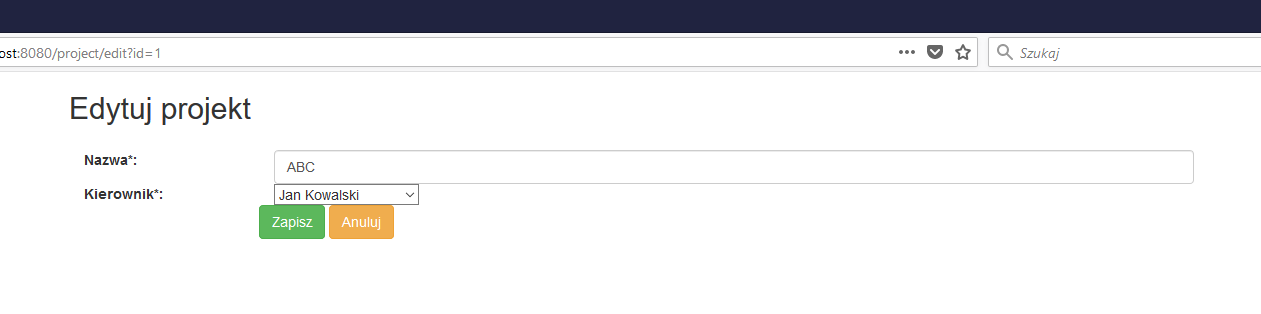
\includegraphics{C:/Users/Kuba/Documents/POLITECHNIKA/9. semestr/Bazy danych/projekt/Dokumentacja/Edycja.PNG}
\caption{}
\end{figure}

\hypertarget{header-n161}{%
\paragraph{Dodawanie projektu}\label{header-n161}}

Na bazie tego samego szablonu, a jedynie dodając nowy punkt dostępu -
otwierający pusty formularz - i modyfikując istniejący - służący do
zapisu - w klasie \emph{ProjectEditResource} można umożliwić
użytkownikowi tworzenie nowych projektów.

\begin{Shaded}
\begin{Highlighting}[]
\AttributeTok{@RequestMapping}\NormalTok{(}\StringTok{"/create"}\NormalTok{)}
\KeywordTok{public} \BuiltInTok{String} \FunctionTok{createProject}\NormalTok{(Model model) \{}
\NormalTok{  ProjectEditDO project = }\KeywordTok{new} \FunctionTok{ProjectEditDO}\NormalTok{();}
\NormalTok{  model.}\FunctionTok{addAttribute}\NormalTok{(}\StringTok{"project"}\NormalTok{, project);}
  \BuiltInTok{List}\NormalTok{<LeaderCandidateDO> leaderCandidates = employeeRepo.}\FunctionTok{findLeaderCandidates}\NormalTok{();}
\NormalTok{  model.}\FunctionTok{addAttribute}\NormalTok{(}\StringTok{"employees"}\NormalTok{, leaderCandidates);}
\NormalTok{  model.}\FunctionTok{addAttribute}\NormalTok{(}\StringTok{"activity"}\NormalTok{, }\StringTok{"Stwórz projekt"}\NormalTok{);}
  \KeywordTok{return} \StringTok{"project-edit"}\NormalTok{;}
\NormalTok{\}}

\AttributeTok{@RequestMapping}\NormalTok{(value = }\StringTok{"/save"}\NormalTok{, method = RequestMethod.}\FunctionTok{POST}\NormalTok{)}
\KeywordTok{public} \BuiltInTok{String} \FunctionTok{saveProject}\NormalTok{(}\AttributeTok{@ModelAttribute}\NormalTok{(}\StringTok{"project"}\NormalTok{) ProjectEditDO projectData) \{}
\NormalTok{  Project project = Optional.}\FunctionTok{ofNullable}\NormalTok{(projectData.}\FunctionTok{getId}\NormalTok{()).}\FunctionTok{map}\NormalTok{(projectRepo::findOne).}\FunctionTok{orElse}\NormalTok{(}\KeywordTok{new} \FunctionTok{Project}\NormalTok{());}
\NormalTok{  project.}\FunctionTok{setName}\NormalTok{(projectData.}\FunctionTok{getName}\NormalTok{());}
  \KeywordTok{if}\NormalTok{ (project.}\FunctionTok{getLeader}\NormalTok{() == }\KeywordTok{null}\NormalTok{)\{}
\NormalTok{    project.}\FunctionTok{setLeader}\NormalTok{(}\FunctionTok{createLeader}\NormalTok{(projectData));}
\NormalTok{    project.}\FunctionTok{setEmployees}\NormalTok{(}\KeywordTok{new} \BuiltInTok{ArrayList}\NormalTok{<>());}
\NormalTok{    projectRepo.}\FunctionTok{save}\NormalTok{(project);}
\NormalTok{  \} }\KeywordTok{else} \KeywordTok{if}\NormalTok{ (project.}\FunctionTok{getLeader}\NormalTok{().}\FunctionTok{getEmployee}\NormalTok{().}\FunctionTok{getId}\NormalTok{() != projectData.}\FunctionTok{getLeaderCandidateId}\NormalTok{()) \{}
\NormalTok{    Leader formerLeader = project.}\FunctionTok{getLeader}\NormalTok{();}
\NormalTok{    project.}\FunctionTok{setLeader}\NormalTok{(}\FunctionTok{createLeader}\NormalTok{(projectData));}
\NormalTok{    projectRepo.}\FunctionTok{save}\NormalTok{(project);}
\NormalTok{    leaderRepo.}\FunctionTok{delete}\NormalTok{(formerLeader);}
\NormalTok{  \} }\KeywordTok{else}\NormalTok{ \{}
\NormalTok{    projectRepo.}\FunctionTok{save}\NormalTok{(project);}
\NormalTok{  \}}
  \KeywordTok{return} \StringTok{"redirect:/project"}\NormalTok{;}
\NormalTok{\}}
\end{Highlighting}
\end{Shaded}

Po naciśnięciu przycisku "Dodaj projekt" można zobaczyć następujący
formularz.

\begin{figure}
\centering
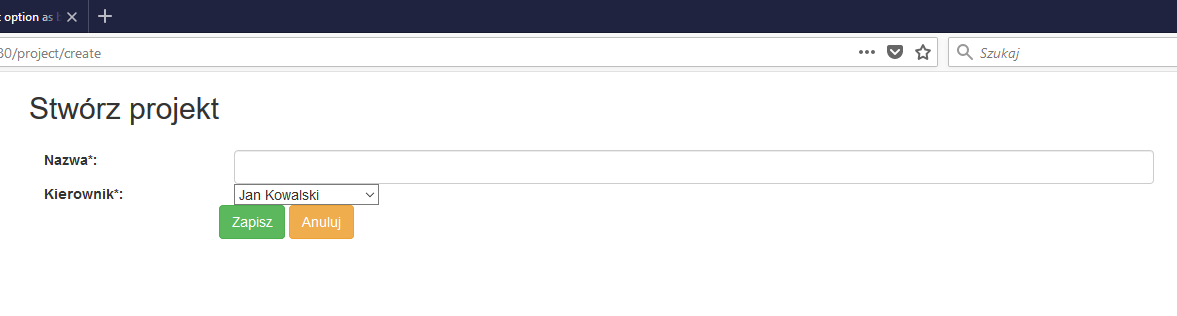
\includegraphics{C:/Users/Kuba/Documents/POLITECHNIKA/9. semestr/Bazy danych/projekt/Dokumentacja/Dodawanie.PNG}
\caption{}
\end{figure}

\hypertarget{header-n169}{%
\subsection{Wdrożenie i testowanie aplikacji}\label{header-n169}}

Rozpoczęcie pracy testowania naszego systemu polega na połączeniu
minimum dwóch maszyn wirtualnych. Donaszego testowania użyliśmy trzech
maszyn wirtualnych uruchomionych na „vmwareworkstation player''.
Następnie na każdej maszynie zainstalowaliśmy systemubuntu oraz
najnowszą wersję MySQL. Kolejnym krokiem jest konfiguracja naszychbaz
danych polegające na wprowadzeniu zewnętrznych ip maszyn wirtualnych
orazuruchomienie replikacji. Działanie takie umożliwi nam replikacje
pomiędzy naszymibazami danych. Ostatnim krokiem zostaje zainstalowanie
naszej aplikacji nakażdej maszynie. Pierwsze uruchomienie naszej
aplikacji na jednej z maszyn,spowoduje stworzenie naszej bazy oraz
dodanie rekordów. Dzięki uruchomionej replikacjidane zostaną wysłane na
inne bazy danych.

Testowanie naszego systemu polega na przetestowaniu trzechakcji:
dodawania, usuwanie oraz edycji naszego rekordu z bazy danych. Wmomencie
dodawania nowego rekordu na jednych z aplikacji, możemy zauważyć, żepo
odświeżeniu aplikacji na innych maszynach spowoduje pojawienie się
nowego rekordu.Niezależnie na której aplikacji dodamy nowy rekord
zostanie on również dodanydo replikowanych baz danych. Podobne
zachowanie możemy zauważyć w momencieusuwania lub edycji rekordu.
Niezależnie na której aplikacji usuniemy lub zedytujemy nasz rekordu, po
odświeżeniu naszych aplikacji zobaczymy usunięty lubz edytowany rekord w
naszych aplikacjach. W podanych źródłach możemy zauważyćdziałanie naszej
replikacji w aplikacji webowej.

· źródło:
\url{https://www.youtube.com/watch?v=RNjxY1Gp_18\&feature=youtu.be}

· źródło:
\url{https://www.youtube.com/watch?v=knksTXE6U4A\&feature=youtu.be}

· źródło:
\url{https://www.youtube.com/watch?v=dE7Ef1QGg0o\&feature=youtu.be}

\hypertarget{header-n180}{%
\subsection{Podsumowanie}\label{header-n180}}

\hypertarget{header-n181}{%
\subsection{Literatura}\label{header-n181}}

\begin{itemize}
\item
  Wrycza S. i in., \emph{Język UML 2.0 w modelowaniu systemów
  informatycznych}, Helion, Gliwice 2005, s. 33-50
\item
  \url{https://dev.mysql.com/doc/refman/5.7/en/mysql-cluster-replication-multi-master.html}
\item
  \url{https://docs.spring.io/spring/docs/5.0.1.RELEASE/spring-framework-reference/core.html\#spring-core}
\item
  \url{http://docs.spring.io/spring-data/jpa/docs/1.10.4.RELEASE/reference/html/}
\item
  \url{https://www.visual-paradigm.com/support/documents/vpuserguide/3563/3564/85378_conceptual,l.html}
\end{itemize}

\end{document}
